\documentclass{article}

\usepackage[margin=1in]{geometry}
\usepackage{wrapfig}
\usepackage{tkz-euclide}
\usepackage{csquotes}
\usepackage{hyperref}
\usepackage{siunitx}

\title{2021 Castro Valley Junior Math Tournament Problems}
\author{}
\date{}

\begin{document}
\maketitle

\section*{Mooving Cow}
Bessie the Cow is $5$ meters north of Farmer John's house.
She starts running east at $2$ meters per second.
After how many seconds will she be exactly $10$ meters away from Farmer John's house?
Express your answer in exact form.

\section*{Cowangle}
\begin{wrapfigure}{r}{0.35\linewidth}
	\vspace{-20pt}
	\centering
	\begin{tikzpicture}
		\tkzDefPoint(110:2){A}
		\tkzDefPoint(180:2){B}
		\tkzDefPoint(0:2){C}

		\tkzDefPointBy[projection=onto B--C](A)
		\tkzGetPoint{X}

		\tkzDrawPolygon(A,B,C)
		\tkzDrawSegment(A,X)
		\tkzLabelPoints[above](A)
		\tkzLabelPoints[left](B)
		\tkzLabelPoints[right](C)
		\tkzLabelPoints[below](X)
		\tkzMarkRightAngle(B,A,C)
		\tkzMarkRightAngle(A,X,C)
		\tkzLabelLine[above left](A,B){$7$}
		\tkzLabelLine[above right](A,C){$10$}
		\tkzLabelLine[right](A,X){?}
	\end{tikzpicture}
	\vspace{-20pt}
\end{wrapfigure}
Bessie the Cow found the following right triangle $ABC$.
The distance from point $A$ to point $B$ is $7$, and the distance from point $A$ to point $C$ is $10$.
$\angle A$ is a right angle, and $\overline{AX}$ is the altitude from point $A$ to side $\overline{BC}$.
What is the length of this altitude (the distance from point $A$ to point $X$)?
Express your answer in exact form.

\section*{Mooish}
Farmer Paul has two types of cows: truthy cows and falsy cows.
Physically, they are indistinguishable.
They all speak mooish, and they can be distinguished by how they answer questions.
The truthy cows always reply truthfully, and the falsy cows always lie.
Bessie had a conversation with three of Farmer Paul's cows: Annabelle, Betsie, and Cornelius.
Here's a translation of the conversation.
\begin{displayquote}
	Bessie: Annabelle, is Betsie truthy or falsy? \\
	Annabelle: Falsy \\
	Bessie: Betsie, are the types of Annabelle and Cornelius different? \\
	Betsie: No. \\
	Bessie: Talkative lot, aren't they? Cornelius, is Betsie truthy or falsy? \\
	Cornelius: Truthy.
\end{displayquote}
What is the type of each cow?

\section*{Green Cows}
Help Bessie the Cow answer the question ``How much grass can a green cow chow if green cows can chow grass?''
Bessie and Elsie both chow grass at constant rates.
If Bessie can chow all the grass in a field in $3$ hours and Elsie can chow all the grass in the same field in $4$ minutes, how long will it take for them to chow all the grass in this field together?
Express your answer in exact form.

\section*{My Cow Ate My Homework}
Bessie the Cow obtained Chloe's math homework again.
While she was enjoying this tasty snack, she noticed one problem that seemed very interesting.
Here's the problem statement:
\begin{displayquote}
	If two real numbers $a$ and $b$ are generate randomly and uniformly such that $-9 < a < 9$ and $-9 < b < 9$, what is the probability that $(a + b)^2 < 2ab + 9$?
	Express your answer in exact form.
\end{displayquote}
Bessie is bad at math, so help her by solving this problem.

\section*{Bullpoop (Look Mom No Proof!)}
Bessie the Cow found a website called \url{vixra.org} which mostly publishes high quality scientific bullpoop.
There's a paper (\url{https://vixra.org/abs/2008.0229}) which presents a simple method that supposedly checks whether integers greater than $5$ are prime.
It makes the following statement without proof:
\begin{displayquote}
    The answer to whether the given numbers are prime numbers is to check that:
    \begin{itemize}
        \item[a)] The numbers are not even numbers (the last digit is not divisible by $2$);
        \item[b)] The last digit of numbers in not $5$;
        \item[c)] The sum of the digits of each of the remaining numbers is not divisible by $3$.
    \end{itemize}
    A number that meets the above criteria is either a prime or a power [of a] prime.   
\end{displayquote}
Disprove this claim.

\section*{Mooshroom Pizza}
\begin{wrapfigure}{r}{0.35\linewidth}
	\vspace{-20pt}
	\centering
	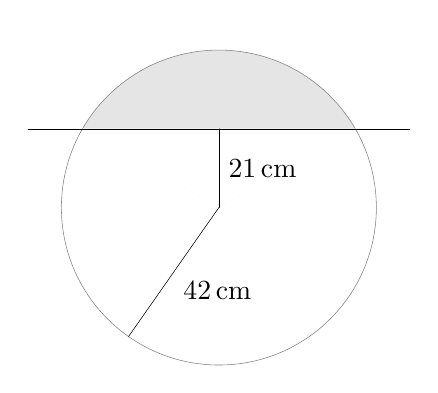
\begin{tikzpicture}[scale=0.5]
		\tkzDefPoint(0,0){A}
		\tkzDefPoint(0,4){B}
		\tkzDefPointBy[rotation=center A angle 60](B)
		\tkzGetPoint{C}
		\tkzDefPointBy[rotation=center A angle -60](B)
		\tkzGetPoint{D}
		\tkzFillSector[rotate,fill=gray!20](A,D)(120)
		\tkzDrawCircle(A,B)
		\tkzDrawPolygon[white,fill=white](A,C,D)
		\tkzDrawLine(C,D)
		\tkzDefMidPoint(C,D)
		\tkzGetPoint{E}
		\tkzDrawSegment(A,E)
		\tkzLabelSegment[right](A,E){$\SI{21}{cm}$}
		\tkzDefPointBy[rotation=center A angle 145](B)
		\tkzGetPoint{F}
		\tkzDrawSegment(A,F)
		\tkzLabelSegment[below right](A,F){\SI{42}{cm}}
	\end{tikzpicture}
	\vspace{-20pt}
\end{wrapfigure}
Farmer John made a mooshroom pizza for the cows.
(Mooshroom pizzas are ethically sourced and don't contain mooshroom meat.
They're called mooshroom pizzas because they contain mushrooms farmed from mooshrooms.)
Bessie tried to slice it, but she failed miserably, resulting in the cut shown in the following figure.
If the radius of the pizza is $\SI{42}{cm}$ cm and the cut is $\SI{21}{cm}$ cm away from the center of the pizza, what is the area of the smaller piece of pizza that was cut off?
Express your answer in exact form.
\end{document}
